\documentclass[a4paper,11pt]{article}

\usepackage{graphicx}
\usepackage{caption}
\usepackage{subcaption}

\begin{document}
\title{\emph{CSC2002S} \\
       Mobile Design \& Development \\
       Phase Two}
\author{Kieren Davies (\textsc{dvskie001})}
\date{19 August 2013}
\maketitle

This assignment documents proposed enhancements to the image viewer application for touchscreen Android devices developed in phase one.

\section{Features}  % 20 marks

The following describes the most significant features which should be added to the image viewer.  These are certainly not the only features which could be added, but they are the ones which are predicted to be most useful.

%\subsection{Gesture control}
%
%Navigation, and other actions introduced below, can be done through natural touch gestures
%
%Naturally afforded gestures reduce the cognitive effort required to perform common actions, and so allow them to be performed more quickly.  This reduces the risk of the user becoming frustrated with the application.
%
%mapping
%convention, least surprise
%pareto principle, most common action, least effort

\subsection{Zoom}

The image can be zoomed in and back out, and panned around while it is zoomed.

Zooming allows the user to observe finer details in a limited area, which can not otherwise be done on a small smartphone screen.

\subsection{Fullscreen}

Fullscreen mode can be toggled, in which all interface controls are hidden and the image covers the whole of the screen.

Using more screen area to display the image allows more detail to be visible when not zoomed, and when zoomed it reduces the need for panning, thereby reducing effort.  Additionally, it increases the signal-to-noise ratio, and permits the screen to be shared without revealing any distracting or private information in the background.

\subsection{Rotate}

Images which have been stored with an incorrect orientation can be rotated left or right in increments of ninety degrees.

Onboard cameras of modern smartphones usually detect the device orientation, so it is uncommon for images to be saved incorrectly, but it may occasionally happen from other sources, such as older cameras or cameraphones.  This can be a considerable frustration to the user, in particular because the correct presentation is so obvious to the human eye.

\subsection{Delete}

Images which the user does not wish to have stored on the device can be permamently deleted.  Undesirable images can frequently result from poor photography or accidental duplicate downloads.

If the image viewer does not provide a mechanism to delete an image immediately, the user may have difficulty finding the same image again in a file browser to delete it.

\subsection{Animations}

Each action is animated to provide feedback to indicate that the action has been performed, but without significantly slowing down interaction or obscuring information.   This includes side-scrolling transitions between images, smooth in-place rotation of the image when it is rotated manually or automatically, and in-place rotation of interface elements which maintain their physical position on the screen when the device is rotated.

According to the aesthetic usability effect this will improve the user experience without altering functionality.

\subsection{Gallery}

Gallery view can be entered, in which all images are displayed in order in a scrollable multi-column list of thumbnails.  Selecting an image returns to the image view with the selected image displayed.

Gallery view provides an overview which allows specific images to be found quickly, instead of slowly searching one-by-one in the image view.

\subsection{Sharing}

An image can be shared as an intent to any installed application which is registered to handle images, in particular social media applications.

As the number of smartphones with continuous internet connectivity grows, it has become increasingly popular to share media digitally, to the point that it has become standard practice to include this feature in Android applications.  Therefore it should be provided in order to conform to user expectations.

\section{Design}  % 40 marks

\begin{figure}[t]
	\begin{subfigure}{0.5\textwidth}
		\centering
		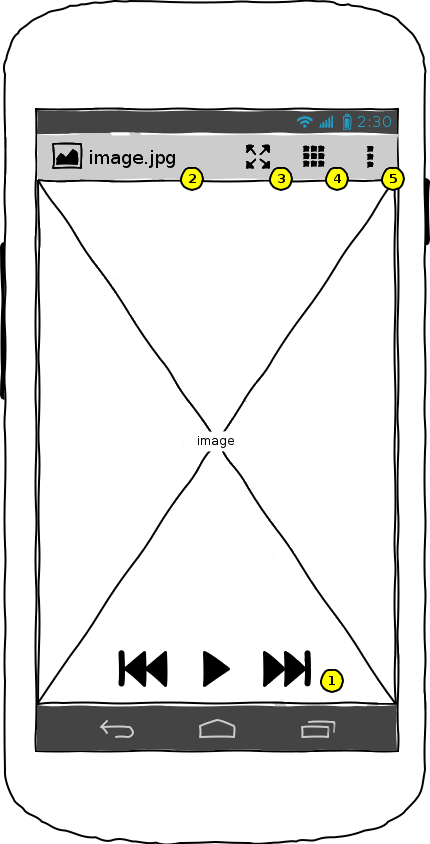
\includegraphics[scale=0.4]{default-portrait}
		\caption{Portrait}
		\label{dp}
	\end{subfigure}
	~
	\begin{subfigure}{0.5\textwidth}
		\centering
		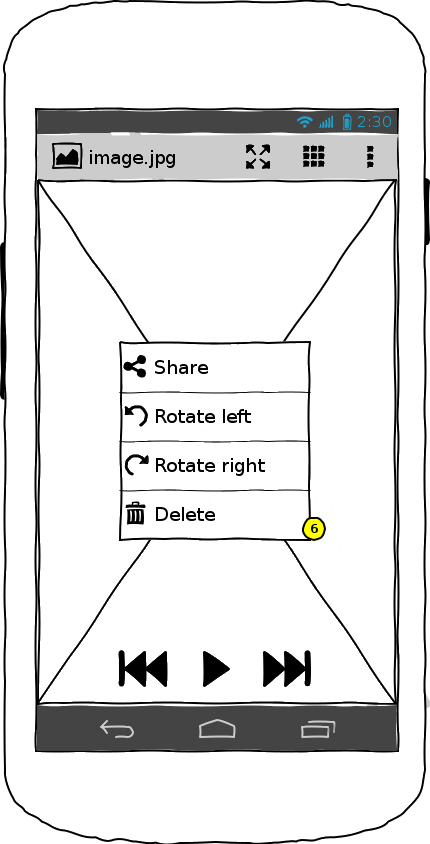
\includegraphics[scale=0.4]{default-portrait-menu}
		\caption{Portrait with menu}
		\label{dpm}
	\end{subfigure}
	
	\begin{subfigure}{\textwidth}
		\centering
		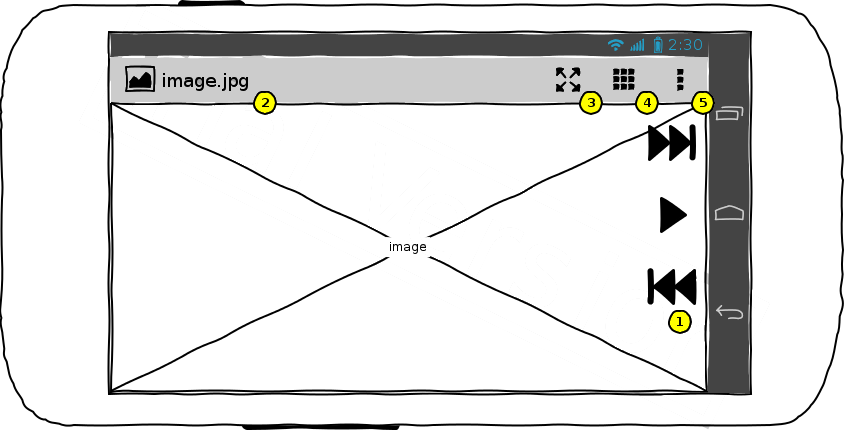
\includegraphics[scale=0.4]{default-landscape}
		\caption{Landscape}
		\label{dl}
	\end{subfigure}
	\caption{Default image view}
	\label{d}
\end{figure}

\begin{figure}[t]
	\centering
	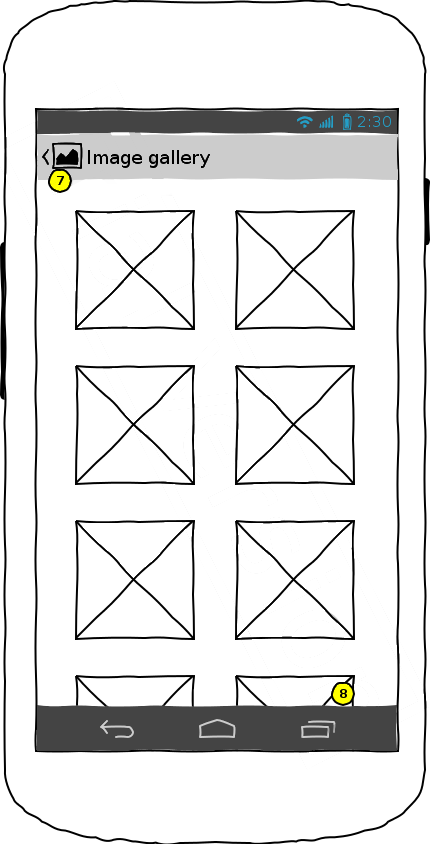
\includegraphics[scale=0.4]{gallery}
	\caption{Gallery view}
	\label{g}
\end{figure}

In portrait mode, the navigation buttons (1) are at the bottom of the screen so as to be clearly visible without obscuring too much of the image, and also easily reachable with a thumb when holding the device.  They use conventional icons to be easily and immediately recognised.  Navigation actions are the most commonly performed actions in an image viewer, 

The action bar shows the image title (2), fullscreen button (3), gallery button (4).  These are all placed here for consistency with Android conventions, and to be very clearly visilble without occupying too much space.  The icons used are standard in Android, so any user familiar with the platform will immediately recognise the purpose of the buttons.  If not, a long press on a button triggers a popup with the button name.
On devices without a physical menu button there is an additional menu overflow button (5), as controlled by the Android operating system.  Pressing this or the hardware menu button causes a menu to be displayed with additional actions (6).  Again, they use standard Android icons.  The items in the menu are less commonly used, so they should be slightly out of the way, as opposed to fullscreen and gallery which are frequently used and should be readily accesible.  This adheres to the principle of least effort.

In landscape orientation, the navigation buttons remain in the same physical location on the screen, so that the users hand does not need to be repositioned.  Even though they are no longer centred, this minor aesthetic change is a fair compromise for consistent physical mapping.

Gestures are the most significant interface feature.  They are swipe to navigate, pinch to zoom, and drag to pan when zoomed.  Navigation is the most common action, so by Pareto's principle these are likely to account for 80\% of the time spent in the application.  Applying the principle of least effort, it is absolutely necessary that these actions are easy both physically and cognitively.  Physically, a coarse gesture is much easier than pressing a comparatively small button, as shown by Hick's law.  Cognitively, gestures map to the instinctive actions of dragging or stretching a sheet of paper.  In combination with transition animations, this provides perfect feedback.

In fullscreen mode only the image is visible, and navigation is done through gestures.  The reasons to hide controls have already been discussed.  Gestures are still enabled because they do not interfere with visibility in any way.  Conversely, fullscreen is not the default view mode because all functionality should be initially visible and exposed.

Gallery view constitutes a mode switch, but this is not problematic because distinctive visual cues give the user sufficien reason to be aware of the mode switch.  Instead of a single large image, in this mode there are two columns of thumbnails which are cropped square.  The action bar now reads \emph{Image gallery}, and the icon (7) doubles as a back button, as per Android convention.  Note that bottom row of images (8) is deliberately only partly visible.  This forces the user to be aware of the ``fold'', that view can be scrolled with a swipe to reveal more image thumbnails.

Note that these designs are only for touchscreen devices with a screen size between 3.5 and 5 inches.  On smaller screens not all buttons may be visible, and those that are will obscure large areas of the image.  On larger screens the application is usable but the large display area is not used optimally, with buttons appearing too small and inconspicuous.

% Affordance
% Mapping
% Constraints (visible constraints)
% Visualising (features made visible) <--
% recognition vs recall
% Memory
% Knowledge \& Chunking
% Pareto principle
% pole
% aue
% pols
% modes, sufficient reason
% feedback
% Hick's law

% \section{Final layout}  % 10 marks

\begin{figure}[p]
	\begin{subfigure}{0.5\textwidth}
		\centering
		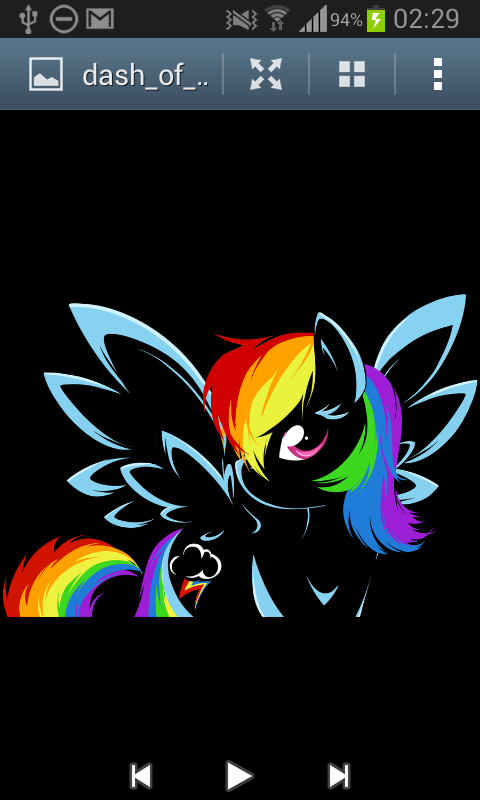
\includegraphics[scale=0.3]{scr1}
		\caption{Portrait}
		\label{flp}
	\end{subfigure}
	~
	\begin{subfigure}{0.5\textwidth}
		\centering
		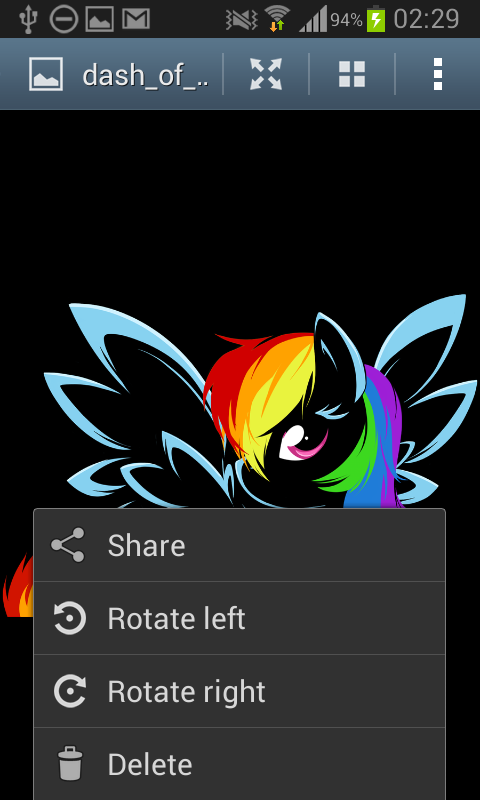
\includegraphics[scale=0.3]{scr2}
		\caption{Portrait with menu}
		\label{flpm}
	\end{subfigure}
	\caption{Final layout screenshots}
	\label{fl}
\end{figure}

% \section{Future features}

% Crop, annotations

\end{document}